\scanpage{38}
\mspage{3}
\textcircled{$\unsure{j_0|i_0}$}
\margin{$\varepsilon_0,\rho'_0$}
\[
\begin{gathered}
\varepsilon_1=\rho'_0(\varepsilon_0)=\rho'_0\varepsilon_0\rho_0'^{-1}\\
\sigma=\rho'_0\varepsilon_0^{-1}\\
\rho_0=\varepsilon_0\rho_0'^{-1}\varepsilon_0\\
\rho_1=\varepsilon_0^2\rho_0'^{-1}\\
\rho'_1=\varepsilon_0\rho'_0\varepsilon_0^{-1}
\end{gathered}
\qquad
\boxed{\begin{gathered}
\rho'_0=(\rho'_0(\varepsilon_0)\varepsilon_0)^2\\
\text{i.e.}\quad\rho'_0=(\rho'_0\varepsilon_0\rho_0'^{-1}\varepsilon_0)^2\\
\text{et}\quad[\rho_0'{}^3\deleted{\unsure{\varepsilon_0\rho'_0}},\varepsilon_0]=1
\end{gathered}}
\]
\uline{NB} On peut se borner à la seule équation abracadabrante:
\[
\unsure{\{}\rho'_0\underbrace{\varepsilon_0\rho_0'^{-1}\varepsilon_0\rho'_0}\varepsilon_0
\underbrace{\rho_0'^{-1}\varepsilon_0^{-1}\rho'_0\varepsilon_0^{-1}\rho_0'^{-1}}\varepsilon_0^{-1}=1
\]
\[
\text{i.e.}\quad[\rho'_0\underbrace{\varepsilon_0\rho_0'^{-1}\varepsilon_0\rho'_0},\varepsilon_0]=1
\]
qui implique
\diagram{\begin{tikzcd}[column sep=small]
\unsure{\varepsilon_0\rho_0'^{-1}\varepsilon_0\rho'_0}\arrow[d,bend right]&\deleted{\text{donc}}\ \rho'_0{}^{\deleted{\unsure{3}}}=(\rho'_0(\varepsilon_0)\varepsilon_0)^2\quad\text{donc}\\
(\unsure{-}\rho'_0(\varepsilon_0)\varepsilon_0)^3&
\end{tikzcd}}
Sym. pour expressions en $\varepsilon_1,\rho'_1$ (relations $(j_1)$)

\textcircled{$h'_0$}\deleted{$\unsure{j_0}$}
\margin{\figure{\begin{tikzpicture}\draw[->] (0,0) .. controls (-.2,1.8) and (-.3,4.8) .. (.4,5.6);\end{tikzpicture}}}
\margin{$\varepsilon_0,\rho_1$\par(\unsure{Ce cas se déduit de} $(h_0)$ par conjugaison par $\varepsilon_0$)\par\uline{NB} Il vaut mieux prendre $\uline{\varepsilon_1,\rho_0}$.}
\[
\begin{gathered}
\varepsilon_1=\rho_1^{-1}(\varepsilon_0)=\rho_1^{-1}\varepsilon_0\rho_1\\
\sigma=\rho_1^{-1}\varepsilon_0\\
\rho_0=\varepsilon_0^{-1}(\rho_1)=\varepsilon_0^{-1}\rho_1\varepsilon_0\\
\rho'_0=\deleted{\unsure{\rho_0}}=\varepsilon_0^{-1}(\rho_1^{-2})=\varepsilon_0^{-1}\rho_1^{-2}\varepsilon_0\\
\rho'_1=\rho_1^{-2}
\end{gathered}
\]
\figure{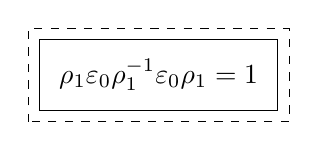
\begin{tikzpicture}\node[draw,inner sep=7pt] (r) {$\rho_1\varepsilon_0\rho_1^{-1}\varepsilon_0\rho_1=1$};\draw[dashed] ([xshift=-4pt,yshift=-4pt]r.south west) rectangle ([xshift=4pt,yshift=4pt]r.north east);\end{tikzpicture}}
Symétriques pour expressions en $(\varepsilon_1,\rho_0)$ (relations $h'_1$)

\textcircled{$j'_0$}
\margin{$\varepsilon_0,\rho'_1$}
\[
\begin{gathered}
\varepsilon_1=\rho_1'^{-1}(\varepsilon_0)=\rho_1'^{-1}\varepsilon_0\rho'_1\\
\sigma=\varepsilon_0^{-1}\rho'_1\\
\rho_1=\varepsilon_0\rho_1'^{-1}\varepsilon_0\\
\rho'_0=\varepsilon_0^{-1}(\rho'_1)=\varepsilon_0^{-1}\rho'_1\varepsilon_0\\
\rho_0=\rho_1'^{-1}\varepsilon_0^2
\end{gathered}
\qquad
\boxed{\begin{gathered}
\rho'_1=(\rho'_1(\varepsilon_0)\varepsilon_0)^2\\
\text{i.e.}\quad\rho'_1=(\rho'_1\varepsilon_0\rho_1'^{-1}\varepsilon_0)^2\\
\text{et}\quad[\rho_1'{}^3,\varepsilon_0]=1
\end{gathered}}
\]
Symétriques pour expressions en $(\varepsilon_1,\rho'_0)$ (relations \deleted{$\unsure{j_1}$} $\unsure{i'_0|j'_0}$)
\mspage{37}
